\begin{figure}[htbp]
  \centering
  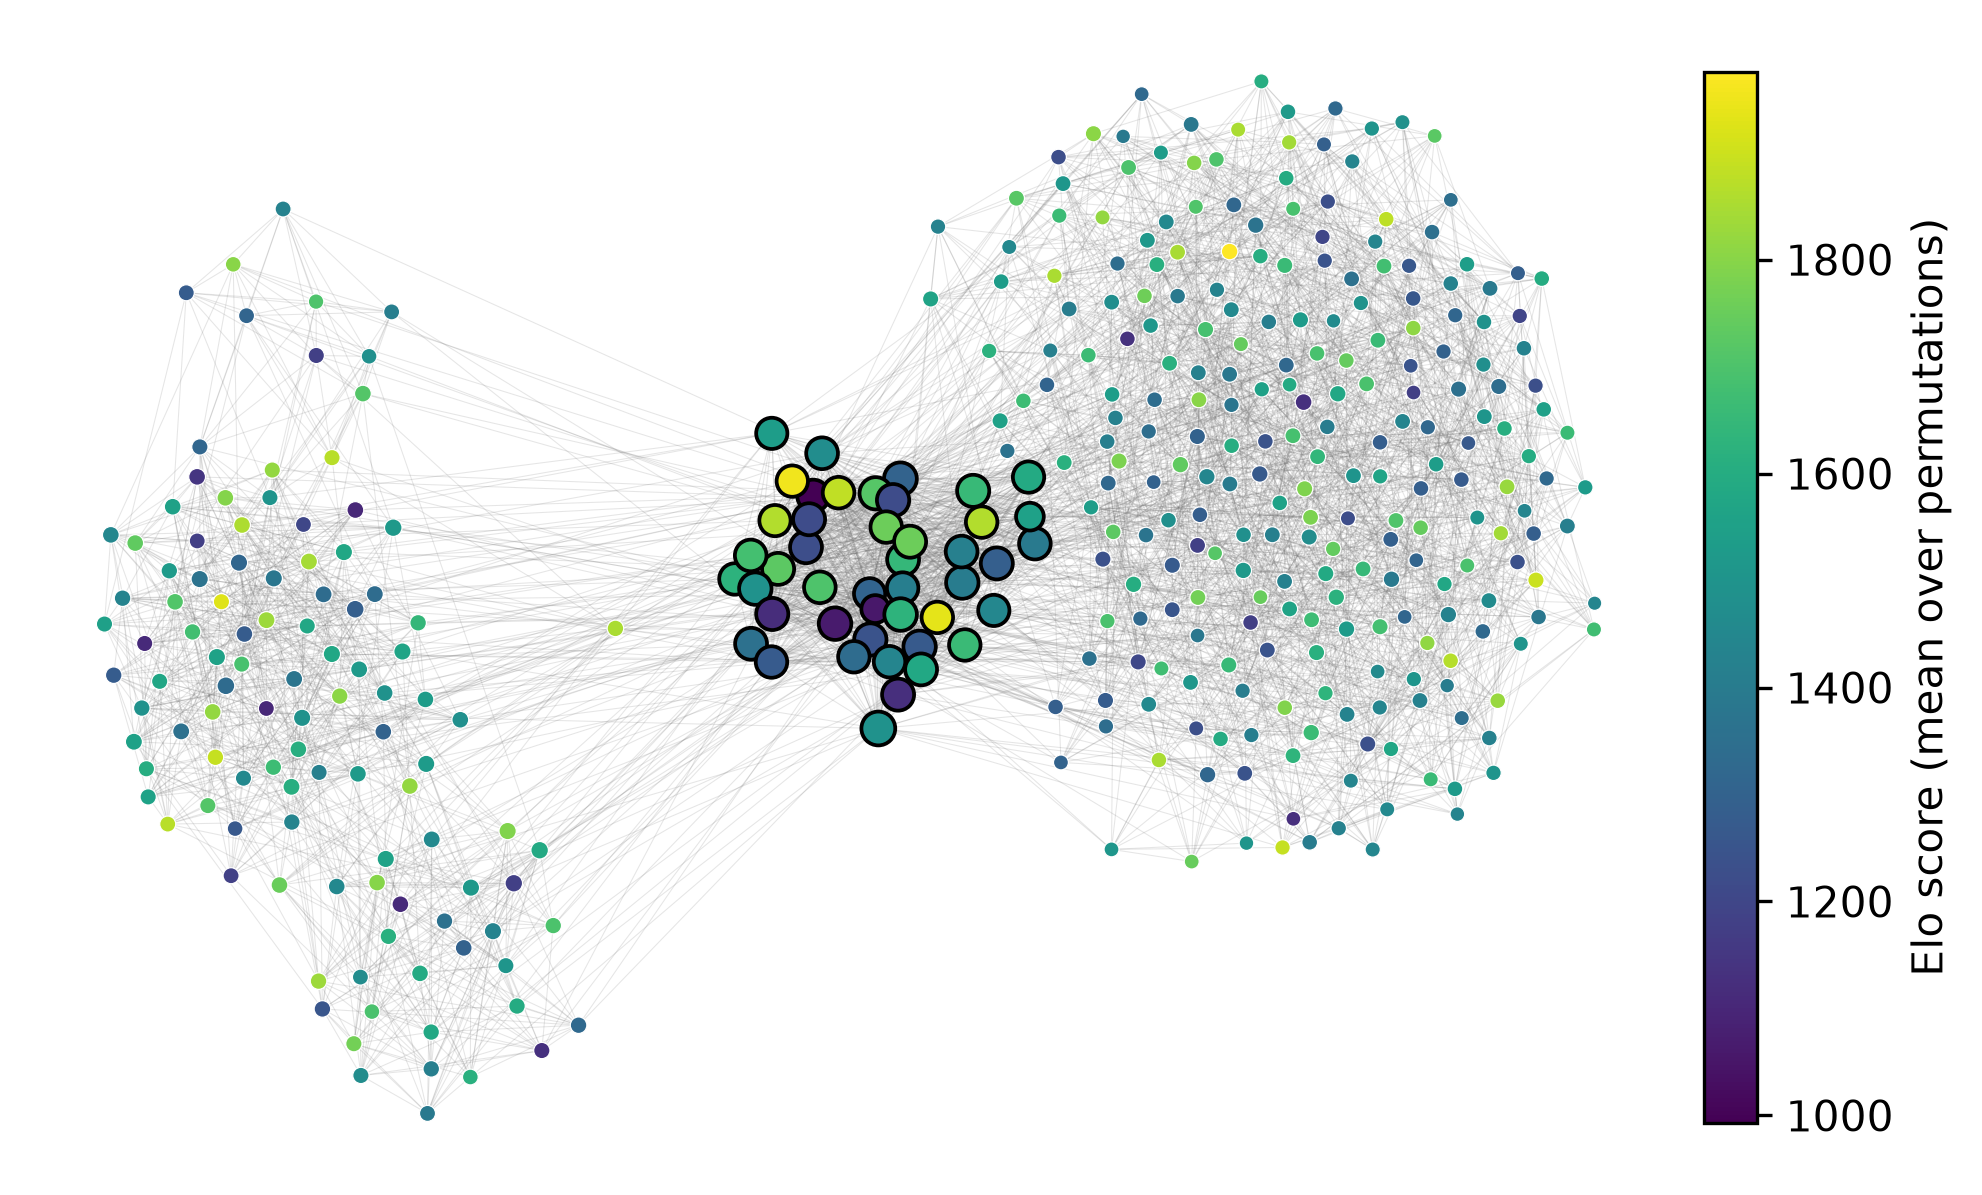
\includegraphics[width=15.00cm]{figures/comparison_graph.png}
  \caption{The comparison graph. Each node represents one of the 397 images. Node size reflects the number of comparisons: from 12 to 122 with median 18. Edges join images judged against each other: 3,787 distinct pairs in 5,562 judgements, which amounts to 4.8\% of the 78,606 possible pairs. Ringed nodes highlight the 45 anchor images, compared more than three times the median number of comparisons. The graph is fully connected. (a) Each image is coloured by batch, in which it was first judged. The pairs judged in the bridging sessions, in which images across batches were evaluated (1,000 judgements in total), are in vermillion; (b) Nodes are coloured by final Elo score.}
  \label{fig:comparison_graph}
\end{figure}
